\section{Conclusion}
\begin{frame}
	\frametitle{Loi faible des grands nombres}
	 Soit $(X_n)_{n \in \boldsymbol{N}}$ une suite de variable aléatoire indépendante et identiquement distribuée de même loi que X (loi mère). Si $\mathbb{E}[|X|] < +\infty$, alors $\overline{X_n} \rightarrow \mathbb{E}[X]$
\end{frame}

\begin{frame}
    \centering
    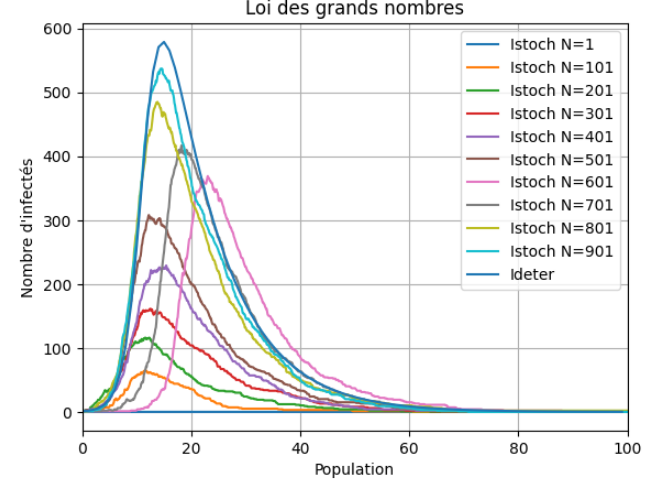
\includegraphics[scale=0.30]{sir_loi_grands_nombres}
\end{frame}
